\documentclass[14pt,aspectratio=169,hyperref={pdftex,unicode},xcolor=dvipsnames]{beamer}
\usepackage[english,russian]{babel}
\usepackage[utf8x]{inputenc}
\usepackage[T2A]{fontenc}
\usepackage{cmap}
\usepackage{paratype}
\usepackage{minted} % для примеров кода (требует параметра -shell-escape)

\usepackage{epigraph}

\usepackage{biblatex}
\usepackage{xurl}
\usepackage{qrcode}
\usepackage{tikz}

\newcommand{\todo}[1]{\textbf{\textcolor{red}{(TODO: #1)}}}
\newcommand{\code}[1]{\mbox{\texttt{#1}}}

\graphicspath{{../images/}}


\usetheme{metropolis}
\usefonttheme[]{professionalfonts}  % запрещаем beamer'у перезаписывать мат. шрифты
\metroset{numbering=fraction}
\metroset{subsectionpage=progressbar}

\setbeamercolor{frametitle}{fg=black}
\setbeamertemplate{frametitle}
{
 \vspace{3mm}\insertframetitle\par
}
\setbeamertemplate{title separator}{}
\setbeamertemplate{footnote separator}{}


\usebackgroundtemplate{
\includegraphics[width=\paperwidth,height=\paperheight]{./common/background_white.jpg}}

\logo{\vspace{-1.2cm}
\includegraphics[width=6mm]{./common/short-v.pdf}\hspace*{1.08\textwidth}}

\institute
{
  \begin{columns}
  \begin{column}{1.5cm}
  
\includegraphics[height=15mm,keepaspectratio]{./common/math-cs.pdf}
  \end{column}
  \begin{column}{4cm}
      Факультет математики и компьютерных наук СПбГУ
  \end{column}
  \end{columns}
}


\begin{document}

\begin{frame}[plain]
  \begin{center}
  \textbf{Вадим Салаватов}

  {\Large\textbf{Реализация мультиплатформенного доступа к файловым хранилищам на языке Kotlin}}

  Выпускная квалификационная работа

  {\small Научный руководитель: профессор, д.ф.-м.н. А.\,С.\,Куликов}

  14 июня 2022
  \end{center}


  \begin{columns}
  \begin{column}{1cm}
  
\includegraphics[height=15mm,keepaspectratio]{./common/math-cs.pdf}
  \end{column}
  \begin{column}{10cm}
    \small
      Факультет математики и~компьютерных наук СПбГУ\\
      Программа <<Современное программирование>>
  \end{column}
  \end{columns}
\end{frame}



\begin{frame}
\frametitle{Введение в предметную область}


% \item О чём здесь вообще речь? Для чего вообще этим всем стоит заниматься?
% \item В чём актуальность работы?
% \item Кто ещё этим занимается, с кем мы будем сравниваться?
% \item Этот слайд необходим для того, чтобы постановка задачи была понятнее.
% \item Вряд ли стоит делать больше двух таких слайдов, иначе вы не успеете рассказать о своей работе.
% \item На введение в предметную область должно уйти не более 15\% времени вашего доклада.
\begin{columns}
  \column{0.62\linewidth}
    \begin{itemize}
    \item Kotlin Multiplatform
    \item Файловые системы
    \item Хотим писать код в общем модуле
    \item Как работать с файловыми хранилищами в веб-браузере?
    \end{itemize}
    
   \column{0.38\linewidth}
    \centering
    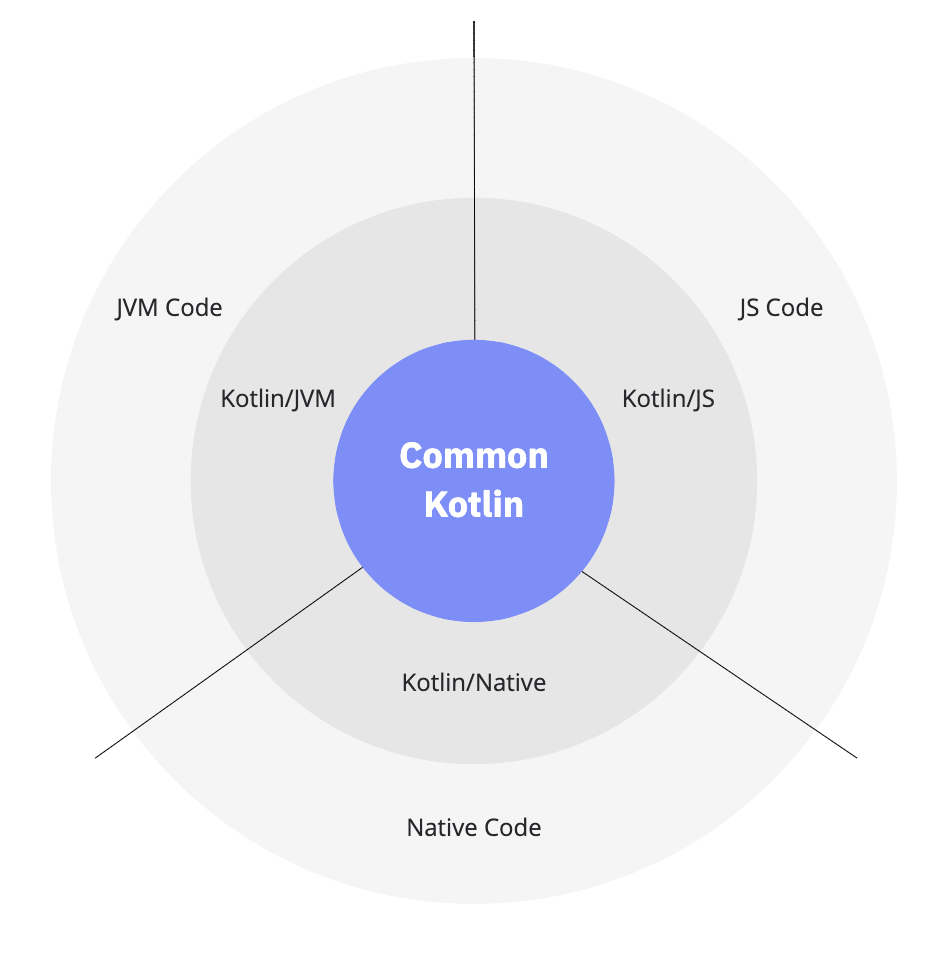
\includegraphics[width=1.07\textwidth,keepaspectratio]{kotlin-multiplatform}
 \end{columns} 
\end{frame}

\begin{frame}{Обзор основных аналогов}

\begin{itemize}
  \item okio
    \begin{itemize}
      \item[+] мультиплатформенность
      \item[+] активно развивается
      \item[+] \texttt{FileSystem}...
      
        \item[-] ...но для JS требует Node.js
      
    \end{itemize}
  \pause 
  \item korlibs/korio
    \begin{itemize}
    \item[+] мультиплатформенность
    \item[+] интерфейс \texttt{VFS}, несколько реализаций
    
    \item[-] последнее обновление почти год назад
    \item[-] перегруженность \texttt{VFS}
    \item[\textpm] для JS есть \texttt{VFS} на основе \texttt{localStorage}
    \end{itemize}
\end{itemize}
\pause
\tikz[remember picture, overlay] \node[anchor=north east] at ([shift={(-0.5,-0.5)}]current page.north east) {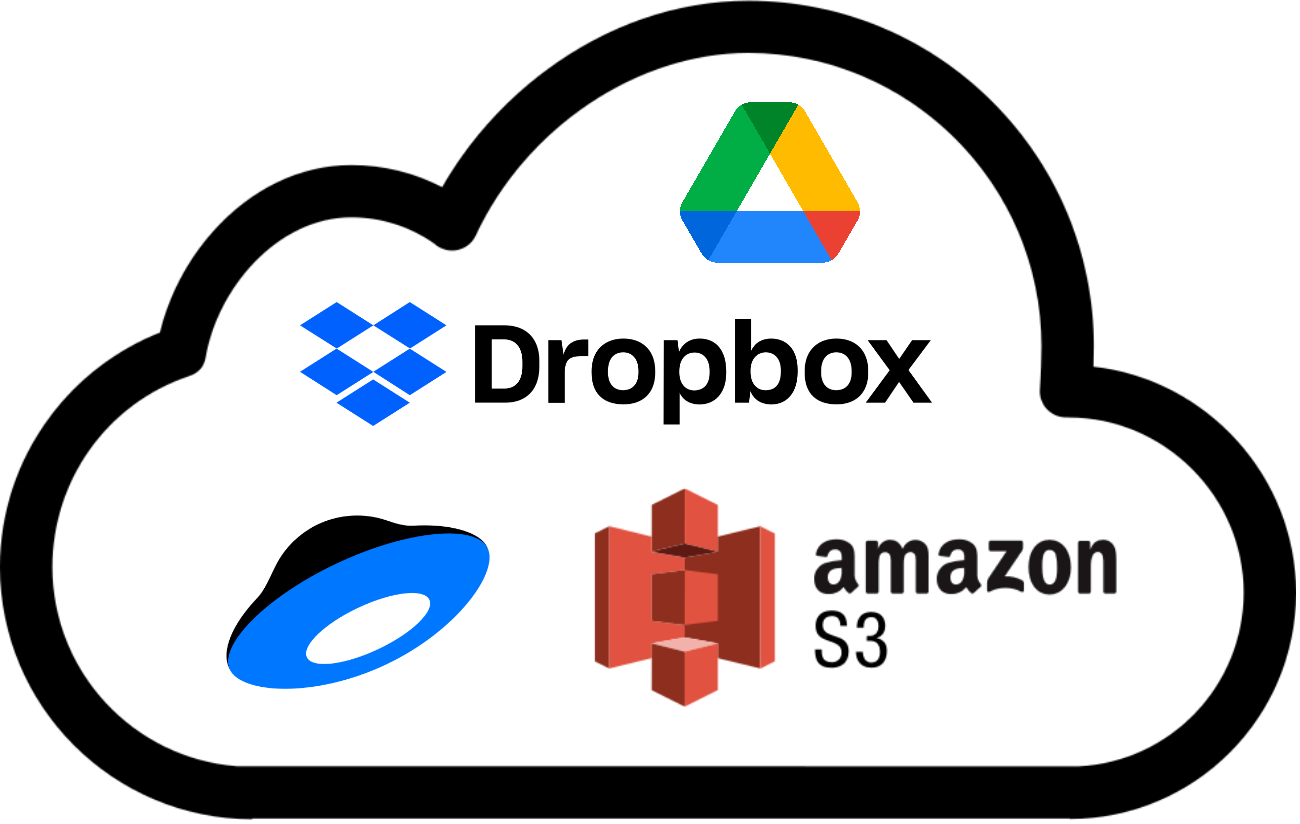
\includegraphics[width=0.35\textwidth]{cloud-services}};
%\begin{tikzpicture}[remember picture,overlay]
  %\tikzset{shift={(current page.center)}}
  %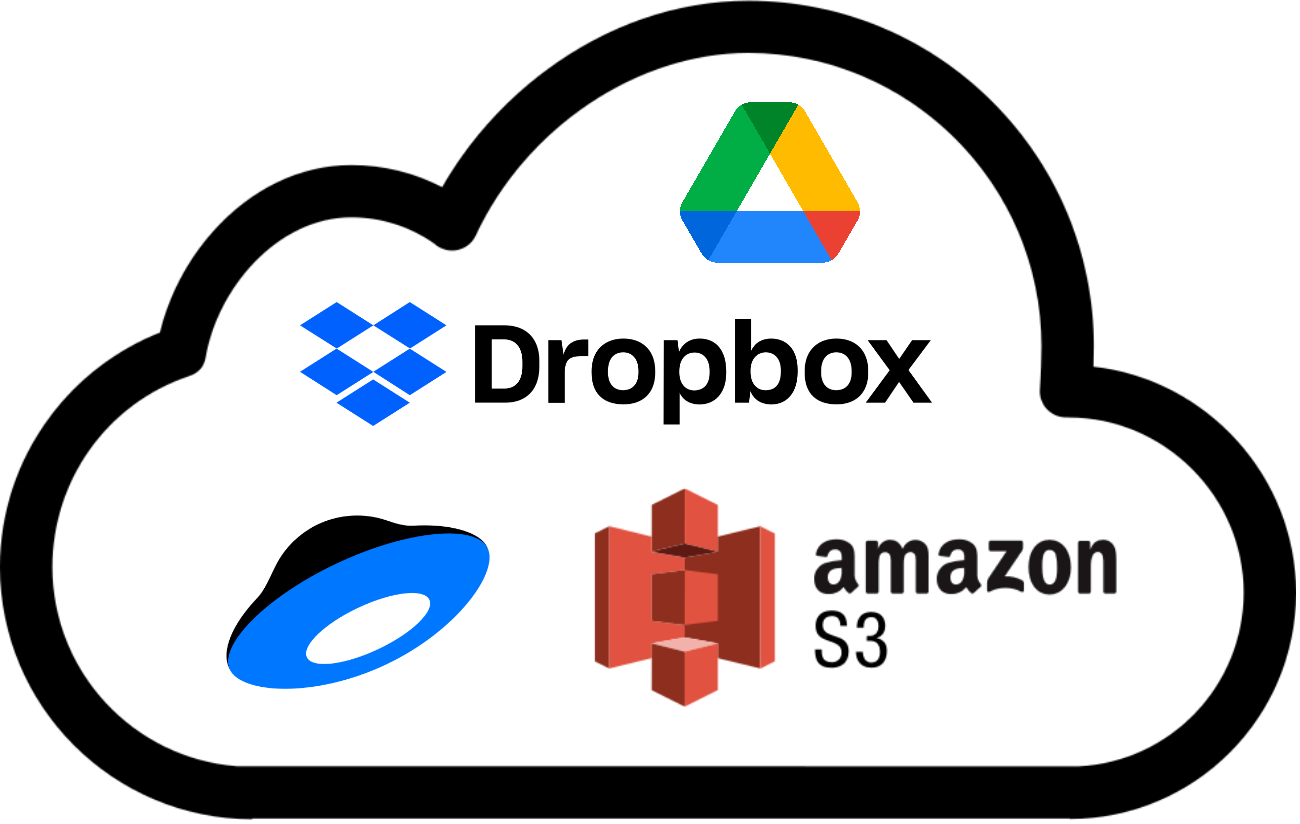
\includegraphics[width=0.4\textwidth]{cloud-services}
  % the picture
%\end{tikzpicture}
\end{frame}

\begin{frame}
\frametitle{Постановка задачи}
\begin{enumerate}
%\item Разработать алгоритм решения задачи путешествующего сейлсмена\footnote{Крайне рекомендуется избегать англицизмов --- старайтесь использовать принятые в~русском языке термины.}, работающий за полиномиальное время.
%\item Построить программную implementation\footnote{Так тоже не надо.}, протестировать её~производительность и сравнить с конкурентами.
%\item Оформить результаты работы в виде доклада на~STOC\footnote{Злоупотреблять аббревиатурами также не стоит, используйте только действительно общепринятые и всем известные сокращения.}.
\item Разработать мультиплатформенную библиотеку для работы с файловыми хранилищами
\item Поддержать платформы JVM, Android, JS (browser)
\item Поддержать как минимум одно облачное хранилище
\item Обеспечить простую расширяемость как в плане поддержки новых хранилищ, так и в плане предоставляемой функциональности
\end{enumerate}
\end{frame}

\begin{frame}{Архитектура библиотеки}
%\small
%   Фильтр минимизирует среднеквадратическое отклонение цвета пикселя.
%  \begin{equation*}\label{eq:wiener_nsr}
%  \hat{Y}(i, j) = \left[ \frac{\hat{H}^*(i, j)}{\left|\hat{H}(i, j)\right|^2 + \frac{S_n(i, j)}{S_s(i, j)}} \right] \times \hat{F}(i, j),
%  \end{equation*}
%\begin{itemize}
%  \item $Y$ -- восстановленное изображение,  $F$ -- наблюдаемое изображение,
%  \item $H$ -- функция рассеивания, $H^*$ --комплексное сопряжение $H$,
%  \item $S_n$ -- энергетический спектр шума -- $\left| \hat{N} \right|^2$,
%  \item $S_s$ -- энергетический спектр исходного изображения -- $\left| \hat{F} \right|^2$,
%  \item $\times$ -- умножение комплексных чисел.
%\end{itemize}
\begin{center}
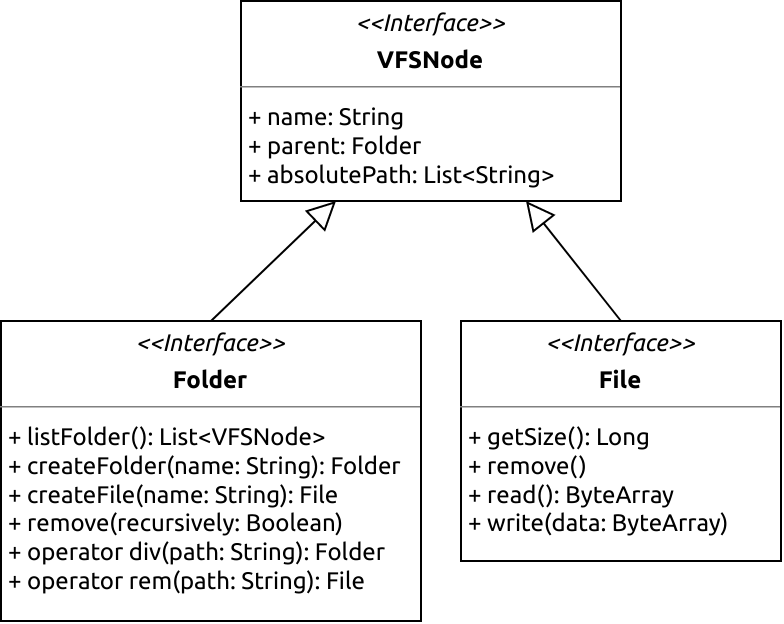
\includegraphics[width=6cm,keepaspectratio]{vfsnode-folder-file}
\hspace{0.2cm}
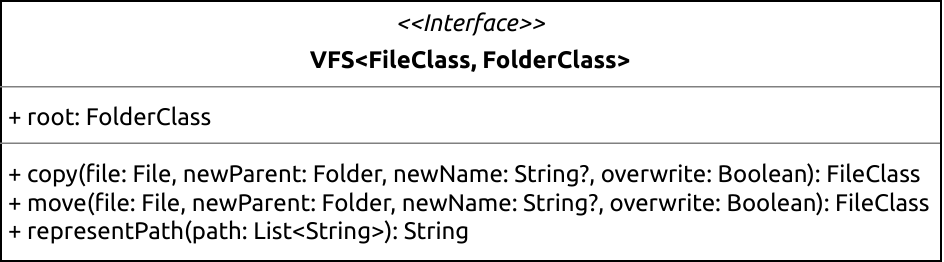
\includegraphics[width=7cm,keepaspectratio]{vfs}

\scriptsize Все методы (кроме \texttt{representPath}) помечены \texttt{suspend}
\end{center}
\end{frame}

%\begin{frame}{SystemFS}
%\begin{center}
%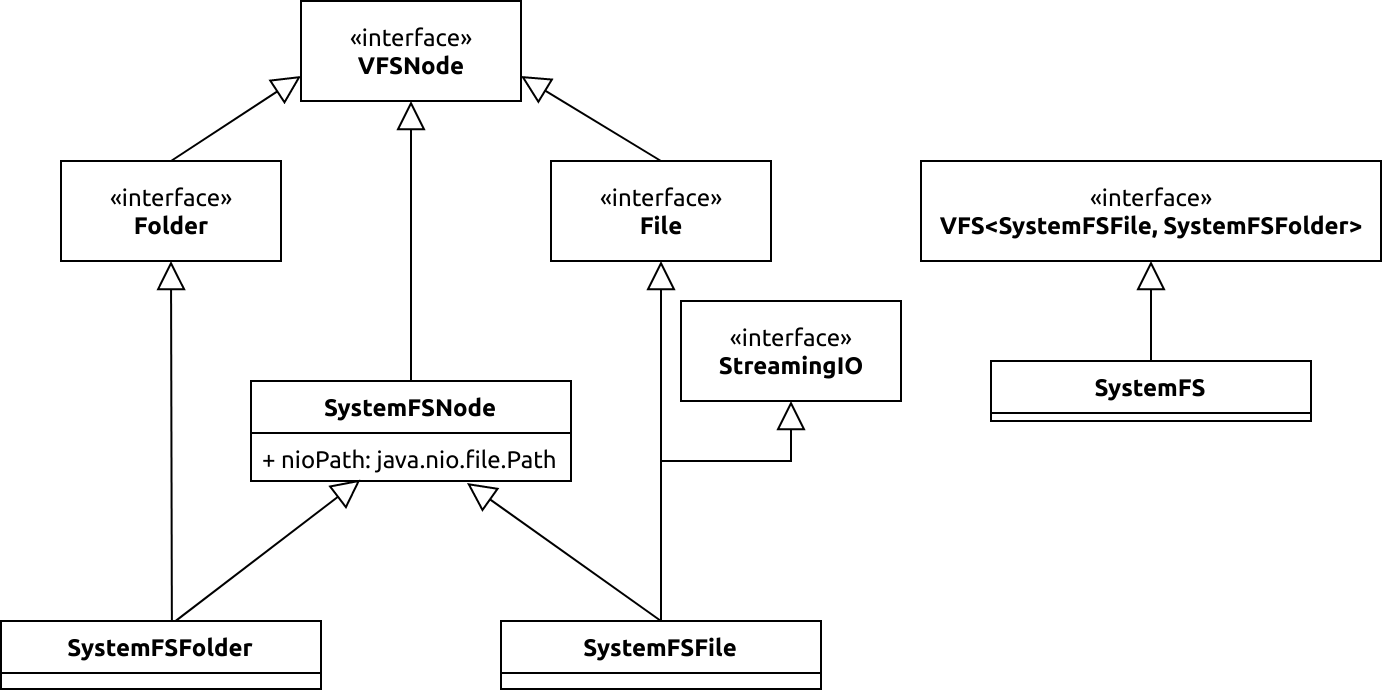
\includegraphics[width=11cm,keepaspectratio]{systemfs-detailed}\\
%\scriptsize доступно на JVM и Android
%\end{center}
%\end{frame}

\begin{frame}{GoogleDriveFS}
\begin{center}
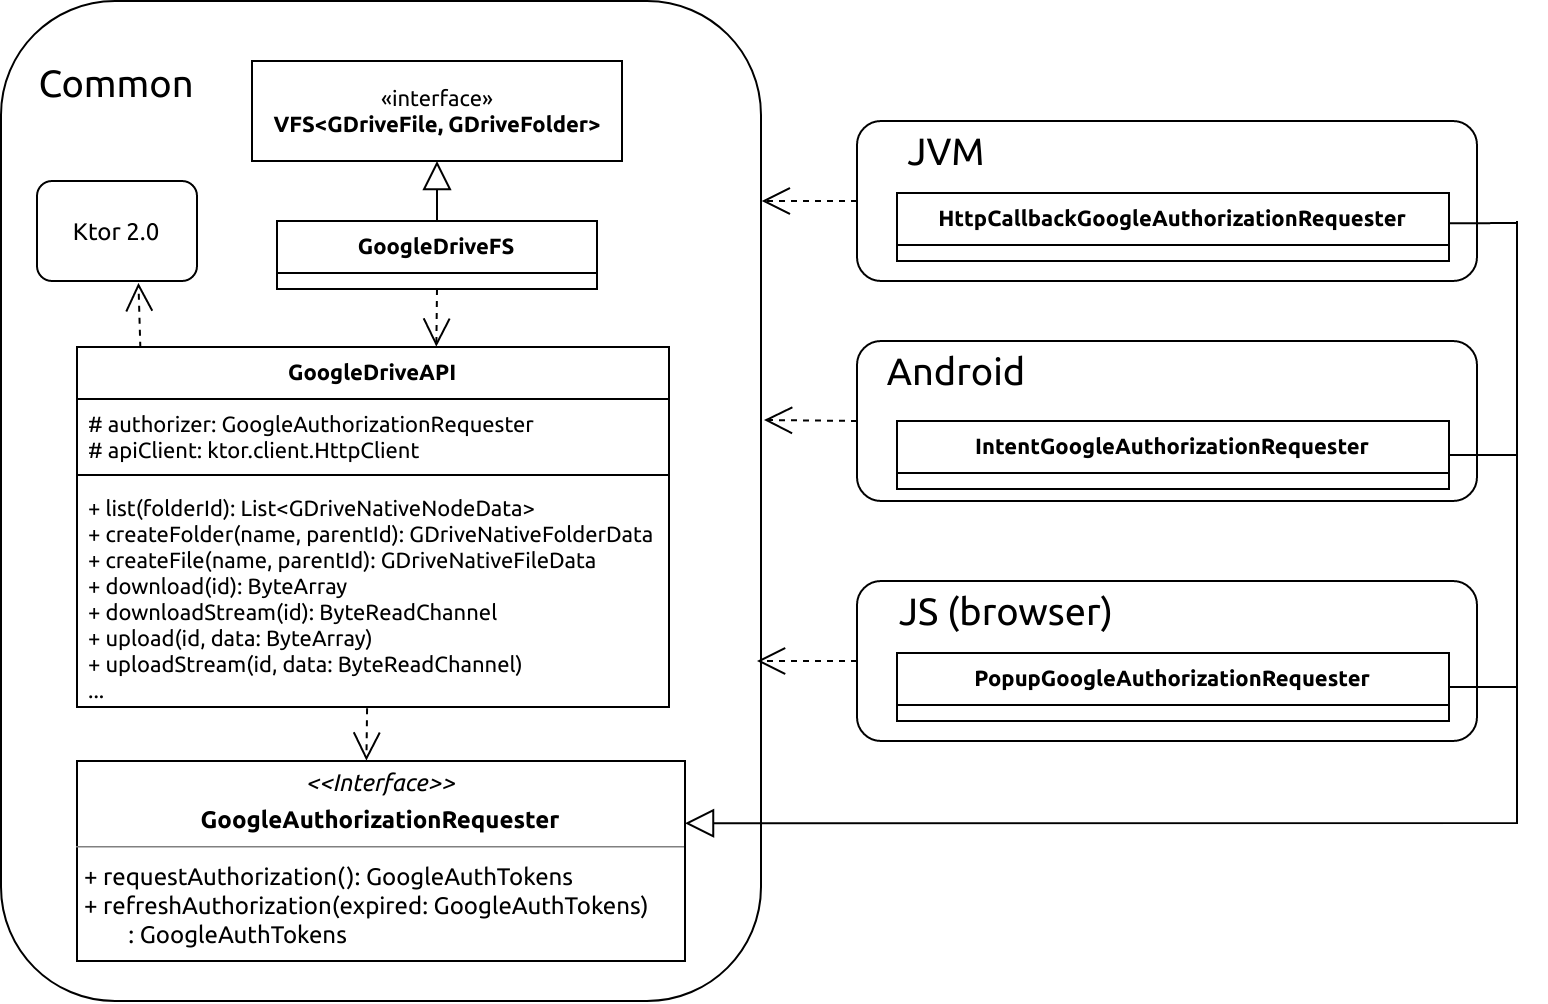
\includegraphics[width=11cm,keepaspectratio]{gdrive-multiplatform-arch}
\end{center}
\end{frame}

%\begin{frame}{SqliteFS}
%  \begin{itemize}
%    \item SQL-эмуляция файловой системы
%    \item Две таблицы: папки и файлы, у файлов есть бинарное содержимое (\texttt{blob})
%    \item Доступно только на Android
%  \end{itemize}
%\end{frame}

%\begin{frame}{Инварианты и гарантии}
%  \begin{itemize}
%    \item Родительская папка корня --- сам корень
%    \item Все методы бросают исключения только типов-наследников VFSException (и, возможно, помеченными некоторыми другими метками)
%    \item Удаление непустой папки только с установленным флагом \texttt{recursively}
%    \item Глобальных ограничений на имена файлов и папок не накладывается --- это может контролировать пользовательский код
%  \end{itemize}
%\end{frame}


\begin{frame}{Расширения}
  \begin{center}
    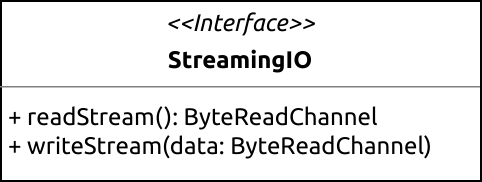
\includegraphics[width=6cm,keepaspectratio]{streamingio}
    %\hspace{0.2cm}
    %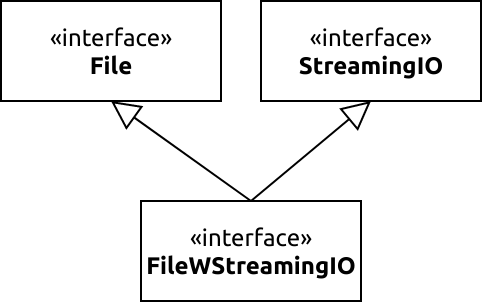
\includegraphics[width=5cm,keepaspectratio]{filewstreamingio}
  \end{center}
  \small SystemFS и GoogleDriveFS реализуют потоковое чтение и запись
\end{frame}
  

\begin{frame}{Сводная таблица поддержанных возможностей}
\centering
\small
\begin{tabular}{|c|c|c|c|c|}
  \cline{2-5}
  \multicolumn{1}{c|}{} & \multicolumn{3}{c|}{Платформа} & Расширения \\
  \hline 
    Название & JVM & Android & JS (browser) & \code{StreamingIO} \\
  \hline 
    \code{SystemFS} & да & да &  & да \\
  \hline 
    \code{GoogleDriveFS} & да & да & да & да \\
  \hline 
    \code{SqliteFS} &  & да &  &  \\
  \hline
\end{tabular}      
%\begin{tabular}{lccc}
%  Хранилище/Платформа & JVM & Android & Web \\
%\hline\hline
%  SystemFS\footnotemark{} & + & + &  \\
%  GoogleDriveFS^\footnotemark[\value{footnote}] & + & + & + \\
%  SqliteFS &  & + & \\
%\end{tabular}
% \footnotetext{есть поддержка \texttt{StreamingIO}}
\end{frame}

\begin{frame}{Приложения на основе библиотеки}
\begin{itemize}
  \item Multieditor\footnote{\url{https://github.com/vsalavatov/multieditor}} --- мультиплатформенный текстовый редактор, работающий на платформах JVM, Android, Web
  \item gdrive-cli\footnote{\url{https://github.com/vsalavatov/gdrive-cli}} --- интерфейс командной строки для работы с содержимым Google Drive, позволяет скачивать и загружать файлы в потоковом режиме
\end{itemize}
\end{frame}

\begin{frame}{Multieditor}
\begin{itemize}
  \item Вся логика работы с файлами в общем модуле
  \item Код графических интерфейсов для JVM и Android написан с помощью Compose в общем для них модуле
  \item Код графического интерфейса для JS (browser) написан на Compose for Web
\end{itemize}
\end{frame}

\begin{frame}{Multieditor JVM}
  \begin{center}
    \only<1>{
      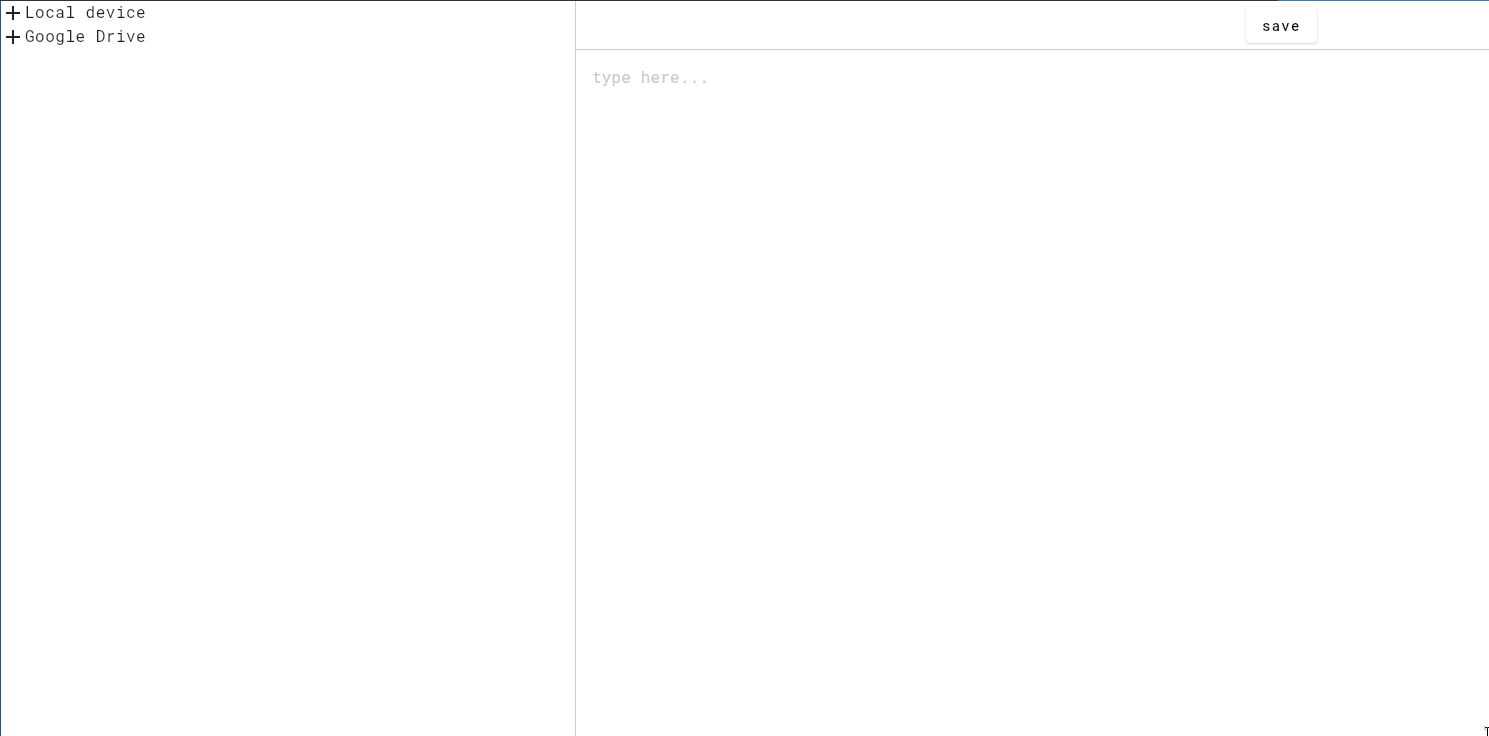
\includegraphics[width=0.92\textwidth,keepaspectratio]{multieditor-jvm-start}
    }
    \only<2>{
      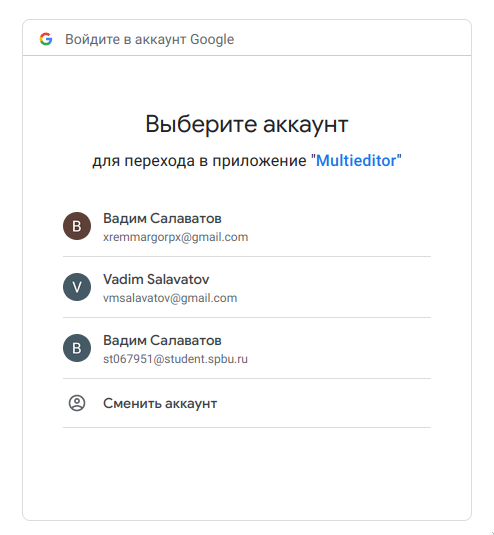
\includegraphics[width=0.45\textwidth,keepaspectratio]{multieditor-jvm-signin}
    }
    \only<3>{
      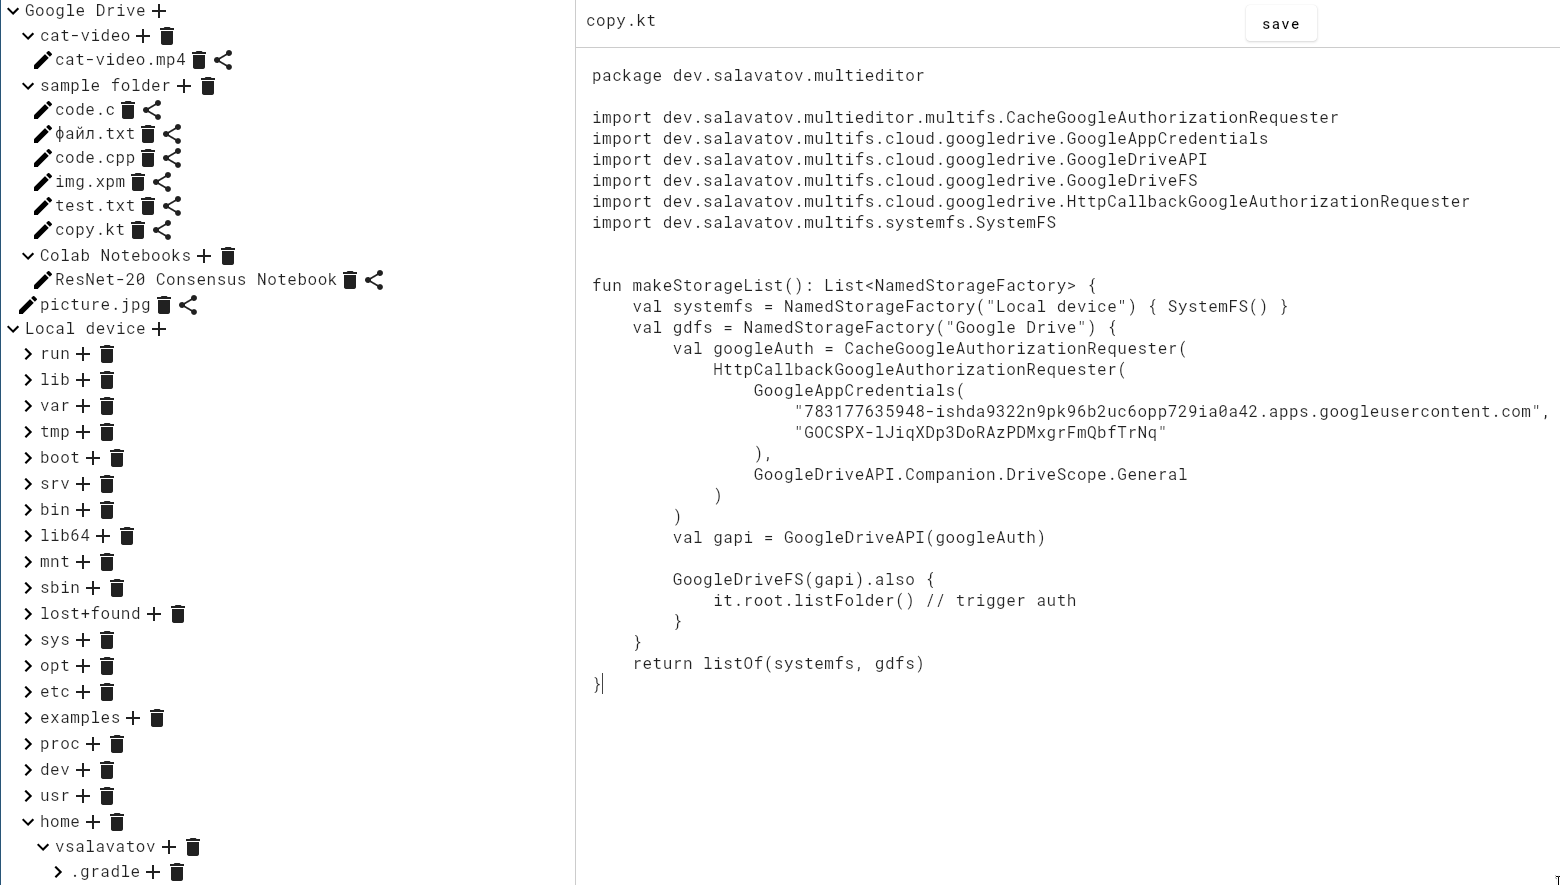
\includegraphics[width=0.92\textwidth,keepaspectratio]{multieditor-jvm}
    }
  \end{center}
\end{frame}


\begin{frame}{Результаты}
  \begin{enumerate}
  \item Реализована библиотека для мультиплатформенной работы с файловыми хранилищами
  \item Поддержаны три хранилища, из которых одно облачное
  \item На основе библиотеки реализовано мультиплатформенное приложение
  \end{enumerate}

  \vspace{2mm}\hrule\vspace{1mm}
    \begin{columns}
      \column{0.85\linewidth}
      \begin{center}
       vmsalavatov@gmail.com, \texttt{@vsalavatov} \\ 
        \url{https://github.com/vsalavatov/multifs}
      \end{center}
      
      \column{0.15\linewidth}
      \begin{center}
        \scalebox{0.82}{\qrcode{https://github.com/vsalavatov/multifs}}
      \end{center}
    \end{columns}  
  
\end{frame}


%%%%%%%%%%%%%%%%%%%%%%%%%% допы

\newcounter{finalframe}
\setcounter{finalframe}{\value{framenumber}}

\begin{frame}
  \begin{center}
  Дополнительные слайды
  \end{center}
\end{frame}


\begin{frame}[fragile]
\frametitle{Как этим пользоваться. Общий код}
\begin{minted}[fontsize=\footnotesize]{kotlin}
typealias Storage = VFS<out File, out Folder>
suspend fun printFiles(folder: Folder) {
  for (node in folder.listFolder()) {
    when (node) {
      is File -> println("${node.name} at ${node.absolutePath}")
      is Folder -> printFiles(node)
    }
  }
}
suspend fun printStorages(storages: List<Storage>) {
  storages.forEach { printFiles(it.root) }
}
\end{minted}
\end{frame}

\begin{frame}[fragile]
\frametitle{Как этим пользоваться. Клиентский код}
\begin{minted}[fontsize=\footnotesize]{kotlin}
fun getStorages(): List<Storage> {
  val systemfs = SystemFS()
  val googleAuth = HttpCallbackGoogleAuthorizationRequester(
                    GoogleAppCredentials(CLIENT_ID, SECRET), 
                    GoogleDriveAPI.Companion.DriveScope.General
                  )
  val gdrivefs = GoogleDriveFS(GoogleDriveAPI(googleAuth))
  return listOf(systemfs, gdrivefs)
}
suspend fun main() {
  printStorages(getStorages())
}
\end{minted}
\end{frame}

\begin{frame}[fragile]
\frametitle{Как этим пользоваться. Расширения}
\begin{minted}[fontsize=\footnotesize]{kotlin}
suspend fun <T> upload(fs: VFS<out T, out Folder>)
        where T : File, T : StreamingIO {
  val file = (fs.root / "folder" / "subfolder" % "file.txt") as T
  val data = ByteReadChannel(
    ByteArray(10_000_000) { it.toByte() }
  )
  file.writeStream(data)
}
...
upload(gdrivefs)
\end{minted}
\end{frame}
  
\begin{frame}{Multieditor Android}
  \begin{center}
    \only<1>{
      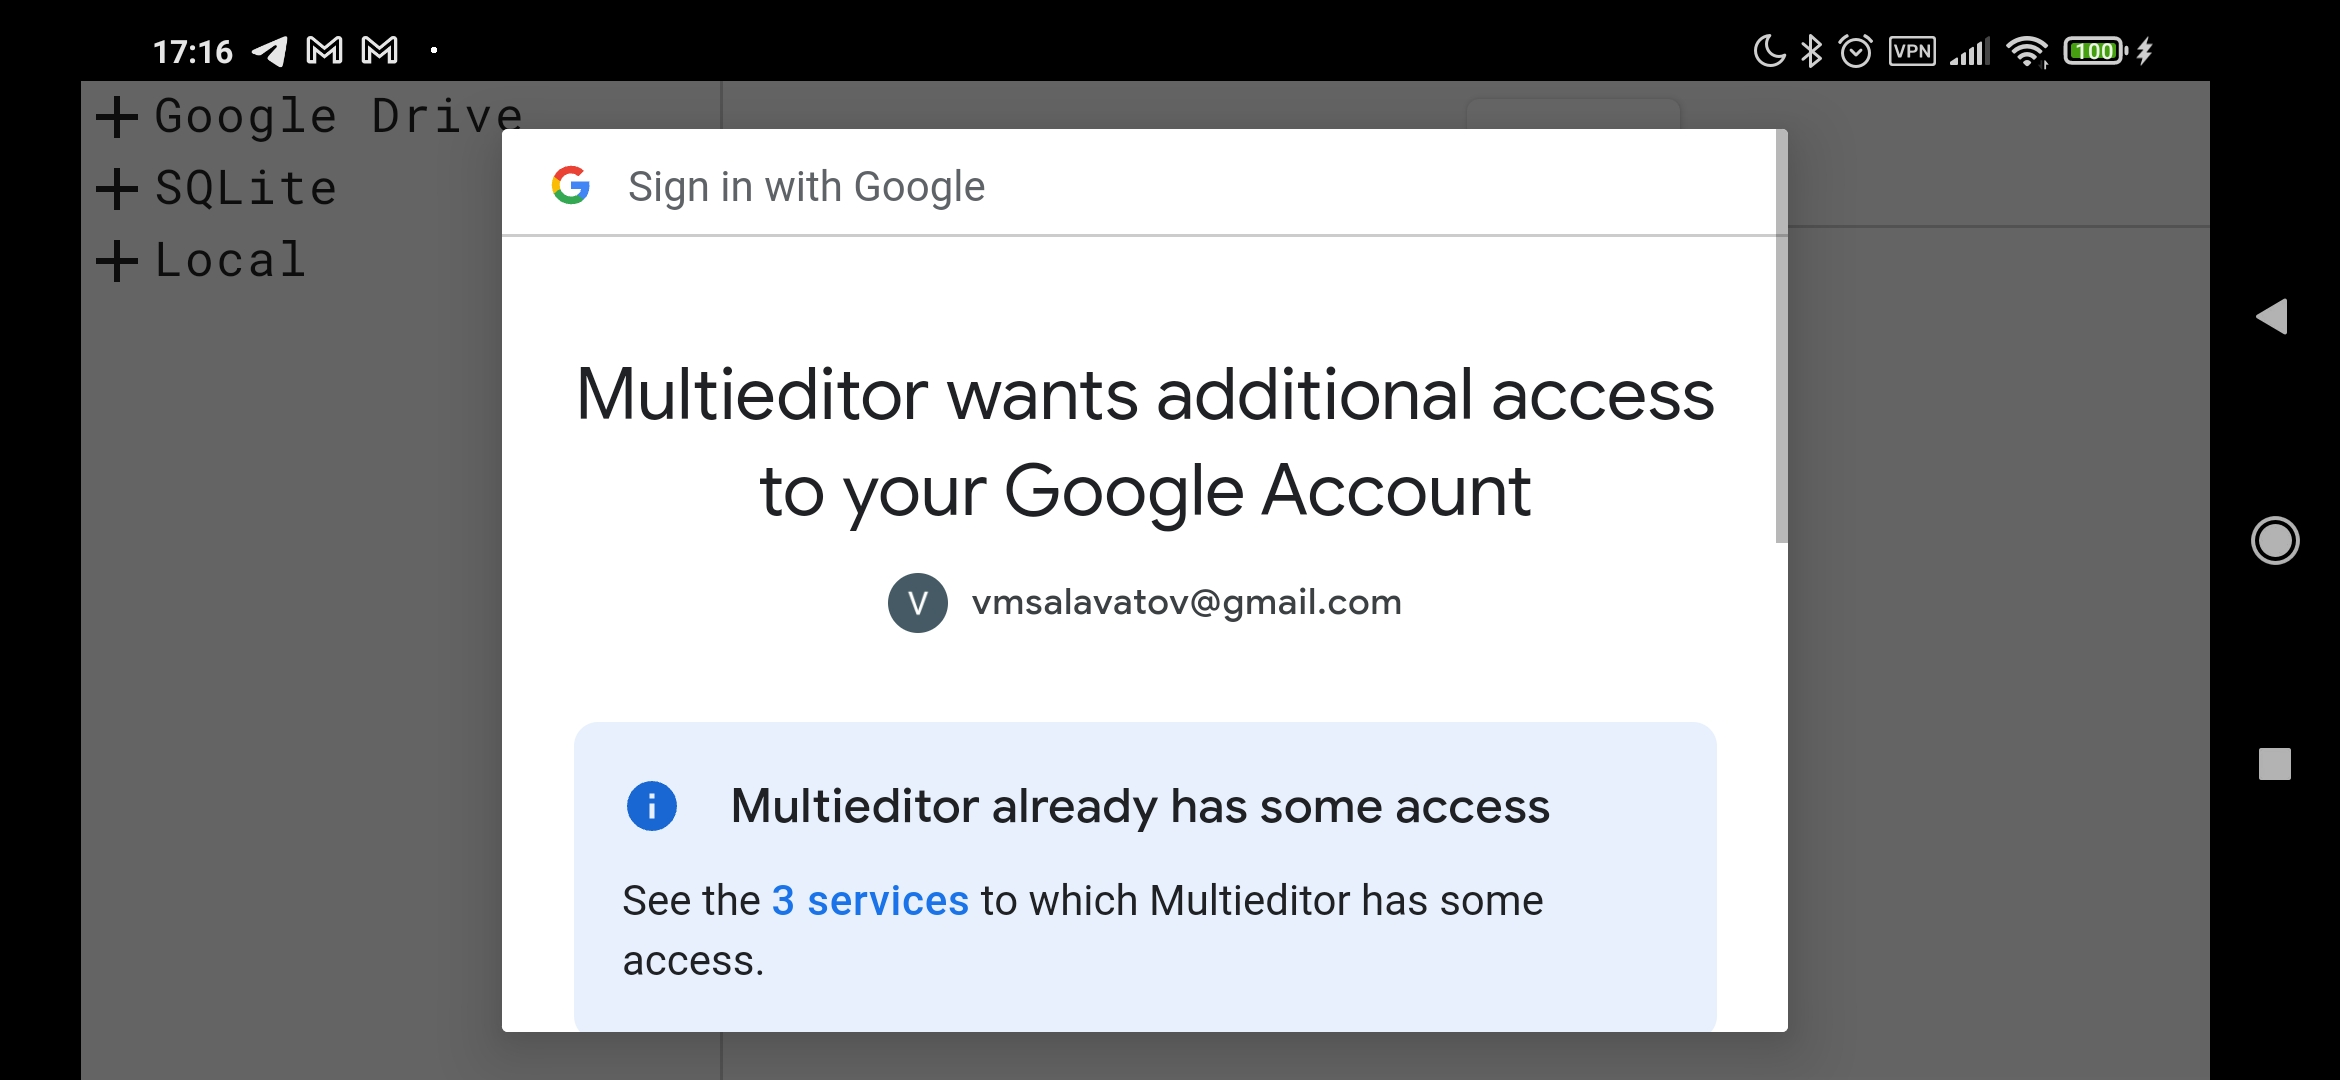
\includegraphics[width=0.8\textwidth,keepaspectratio]{multieditor-android-signin}
    }
    \only<2>{
      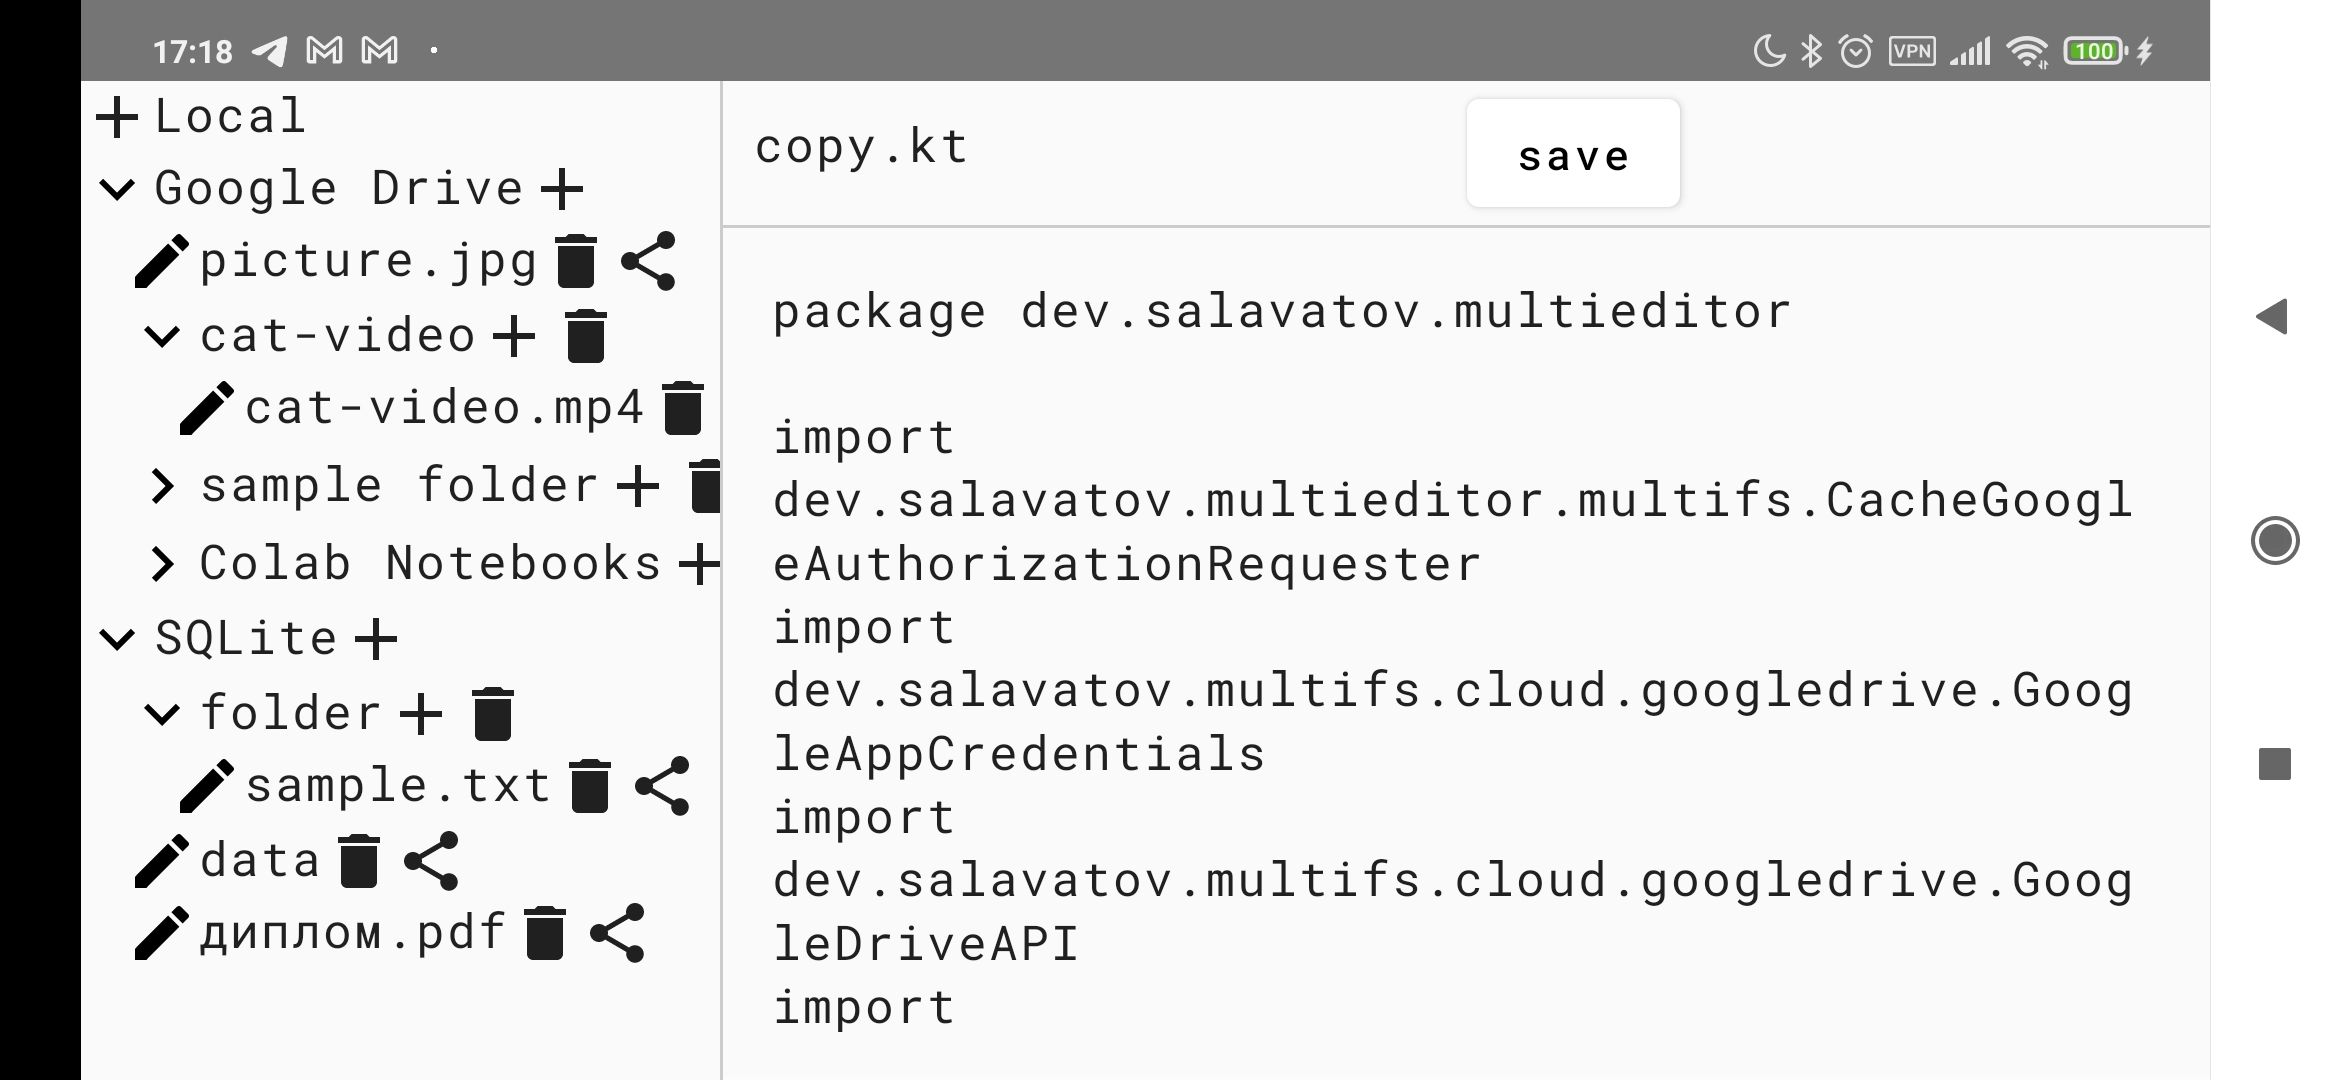
\includegraphics[width=0.8\textwidth,keepaspectratio]{multieditor-android}
    }
  \end{center}
\end{frame}

\begin{frame}{Multieditor Web}
  \begin{center}
    \only<1>{
      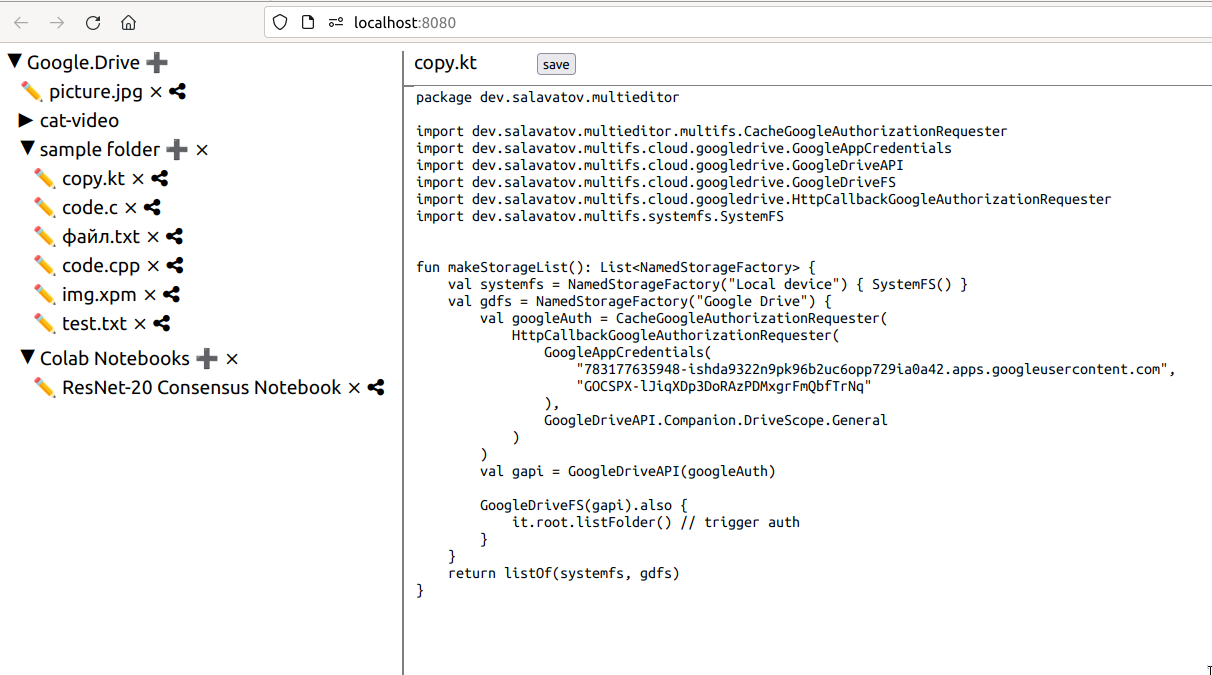
\includegraphics[width=0.92\textwidth,keepaspectratio]{multieditor-web}
    }
  \end{center}
\end{frame}

\setcounter{framenumber}{\value{finalframe}}

%\begin{frame}[fragile]
%\frametitle{Задача 2: код на языке программирования\footnote{Увлекаться кодом на слайдах не стоит, зато структурные и иные диаграммы обычно смотрятся хорошо.}}
%\begin{minted}{kotlin}
%fun main() {
%  val name = "stranger"
%  println("Hi, $name!")
%  print("Current count:")
%  for (i in 0..10) {
%    print(" $i")
%  }
%}
%\end{minted}
%\end{frame}

%\begin{frame}{Задача 2: результаты измерений в таблице}
%\centering
%\begin{tabular}{lccc}
%  Имя & Работа 1 & Работа 2 & Итог \\
%\hline\hline
%  Алиса & 8.0 & 9.0 & 8.5 \\
%  Боб & 9.0 & 9.8 & 9.4 \\
%  Чак & 9.1 & 9.3 & 9.2 \\
%\end{tabular}
%
%\begin{block}{Пояснения к таблице}
%  \begin{itemize}
%  \item Таблицы могут требовать пояснений.
%  \item Что это за величины? Откуда они взялись?
%  \item Какие выводы можно сделать?
%  \end{itemize}
%\end{block}
%
%\end{frame}


%\begin{frame}
%\frametitle{Задача 2: результаты сравнения с конкурентами\footnote{Понятна ли ваша диаграмма? Не забыли ли вы легенду?}\footnote{Контрастно ли изображение? Помните, на проекторе всё может выглядеть хуже.}}
%\begin{center}
%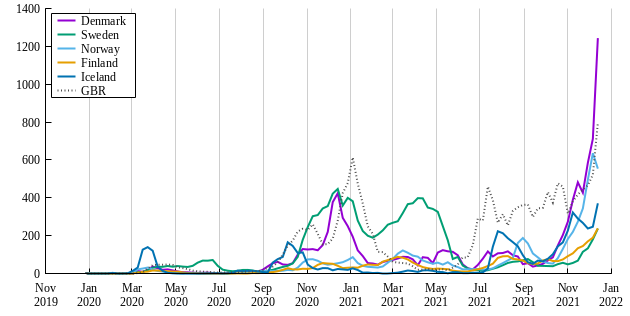
\includegraphics[width=11cm]{images/graph.png}
%\end{center}
%\end{frame}

%\begin{frame}
%\frametitle{Задача 3: основные трудности}
%\begin{itemize}
%\item Мы всё классно сделали, но рецензенты STOC сформулировали ряд претензий к~работе, обозвали нас идиотами и отказались пускать на конференцию.
%\item Все замечания были исправлены, попробуем FOCS\footnote{Не забывайте про нежелательность англицизмов и аббревиатур.}!
%\end{itemize}
%
%\end{frame}

%\begin{frame}
%\frametitle{Дополнительный слайд по работе в целом\footnote{Кстати, слайды с длинными перечислениями выглядят плохо. Старайтесь их избегать.}}
%\begin{itemize}
%\item Освоенные и применённые технологии
%\item Информация о внедрении
%\item Полученные в ходе выполнения работы навыки
%\item Вынесенные уроки
%\item Реальные планы на будущее (не надо фантазировать!)
%\item Ссылки на цитированную литературу --- их можно вынести в конец слайдов, но во время доклада не показывать.
%\end{itemize}
%\end{frame}

\end{document}
